\chapter{Results and Experiments} % Main chapter title

\label{chapter:observer_results} % Change X to a consecutive number; for referencing this chapter elsewhere, use \ref{ChapterX}

\lhead{Chapter 4. \emph{Results and Experiments}} % Change X to a consecutive number; this is for the header on each page - perhaps a shortened title

This chapter presents an experiment used to evaluate the intention recognition capacity of our system. Section~\ref{sec:observer_experiment-case_study} introduces our case study, where we decided to compare the prediction of our system with those of humans. Section~\ref{sec:observer_experiment-experiment} explains how the experiment was actually conducted. We show and discuss our results in section~\ref{sec:observer_experiment-discussion}.


\section{Case Study}
\label{sec:observer_experiment-case_study}
\subsection{Study Description}

Evaluating the capacity of the system to estimate human intentions is not easy, since intentions are not directly observable. A possible solution, as shown in~\cite{baker2014modeling}, is comparing the estimation of human intentions, performed by other humans, with the predictions of our system. In order to perform this comparison we created a user study where we showed participants several videos, asking them to estimate the likelihood of a set of intentions  for each video, and collected their results. The same tests where simulated on the system, streaming as input a sequence of observations  corresponding to the actions shown in the video (e.g. if the video shows a human approaching the table, we will stream to the system a trajectory of coordinates that leads to the table position). All of the test videos ended in a situation of ambiguity. For example, in one test we showed a human approaching a table with different objects, and stopped the video before users could see which object the human wanted to take. Some videos include more information than others, like comments by humans or situations that help to disambiguate the intention. 

We have performed an equivalence test, comparing users' intentions predictions with those of the system, following the two one-sided tests (TOST) approach. We choose as a threshold for equivalence the standard deviation $\sigma$ of the users' answers. The idea behind this choice is that, if the system's answers are closer than a standard deviation to the average human answers, its predictions are comparable to an average human answer from our user group. 

We defined our hypothesis as follow: 
\begin{itemize}
\item $H_0$: $\mu_{hi}-\mu_{si}\leq-\sigma_{hi}$ \; \text{OR} \; $\mu_{hi}-\mu_{si}\geq\sigma_{hi}$ 
\item $H_A$: $-\sigma_{hi}<\mu_{hi}-\mu_{si}<\sigma_{hi}$  
\end{itemize}
where $\mu_{hi}$ and $\mu_{ri}$ are the human average and the system's answer for test $i$, $\sigma_{hi}$ is the variance of the human answers for test $i$.

We have performed tests to evaluate: a) prediction in absence of clues, b) prediction in the presence of contextual clues, c) prediction in the presence of belief state clues.

We built a household environment with a fixed set of furniture: a \textit{Kitchen Shelf}, a \textit{Table}, a \textit{Sofa}, and a \textit{Chair}. In this environment, we created two scenarios, composed by several tests, with two agents, \textit{Max} and \textit{Bob}, performing different actions. Each scenario contained a set of objects, and a constrained set of intentions. For the tests related to belief states, we start by showing the users a specific sequence of events, allowing them to build a mental model of the agents. A corresponding simulated sequence will be streamed to the system for this test.
We will describe in details the two scenarios and the relative tests.

\subsection{Cookie Scenario}
\begin{itemize}
\item Objects: a \textit{Cookie Box}, a \textit{Mug}, and a \textit{Bottle of Water} were placed on the \textit{Table}, close to each other. A pack of \textit{Cookies} was placed on the \textit{Kitchen Shelf}. The \textit{Cookie Box} could contain, or not, \textit{Cookies}.
\item Intentions: \textit{Eating a Cookie}, \textit{Drinking Water}, \textit{Reading the Book}.
\item Tests:
\begin{itemize}
	\item \textit{No Clues}: \textit{Max} approaches the \textit{Table}.
    \item \textit{Contextual Clues}: \textit{Max} approaches the \textit{Table} commenting on the warmth of the day.
	\item \textit{Divergent Belief Max}: \textit{Max} approaches the \textit{Table}.
	\item \textit{Divergent Belief Bob}: \textit{Bob} approaches the \textit{Table}.
\end{itemize}
\item  \textit{Divergent Belief Event}:  \textit{Max} and \textit{Bob} are chatting on the \textit{Sofa}. Max eats the last \textit{Cookie} from the \textit{Cookie Box} before closing it and leaving. While \textit{Max} is away, \textit{Bob} takes \textit{Cookies} from the \textit{Kitchen Shelf}, fills the \textit{Cookie Box} with them, and closes it, before leaving.
\end{itemize}

The \textit{Divergent Belief Event} was shown to the users (and its simulation streamed to the system) between the \textit{Contextual Clues} and the \textit{Divergent Belief Max} events. 


We deliberately included an intention, \textit{Reading the Book}, without placing a book in the visible environment, introducing a confusing element in the scenario. This scenario can be seen in figure~\ref{fig:observer_experiments-cookie}.


 \begin{figure}[ht!]
	\centering
	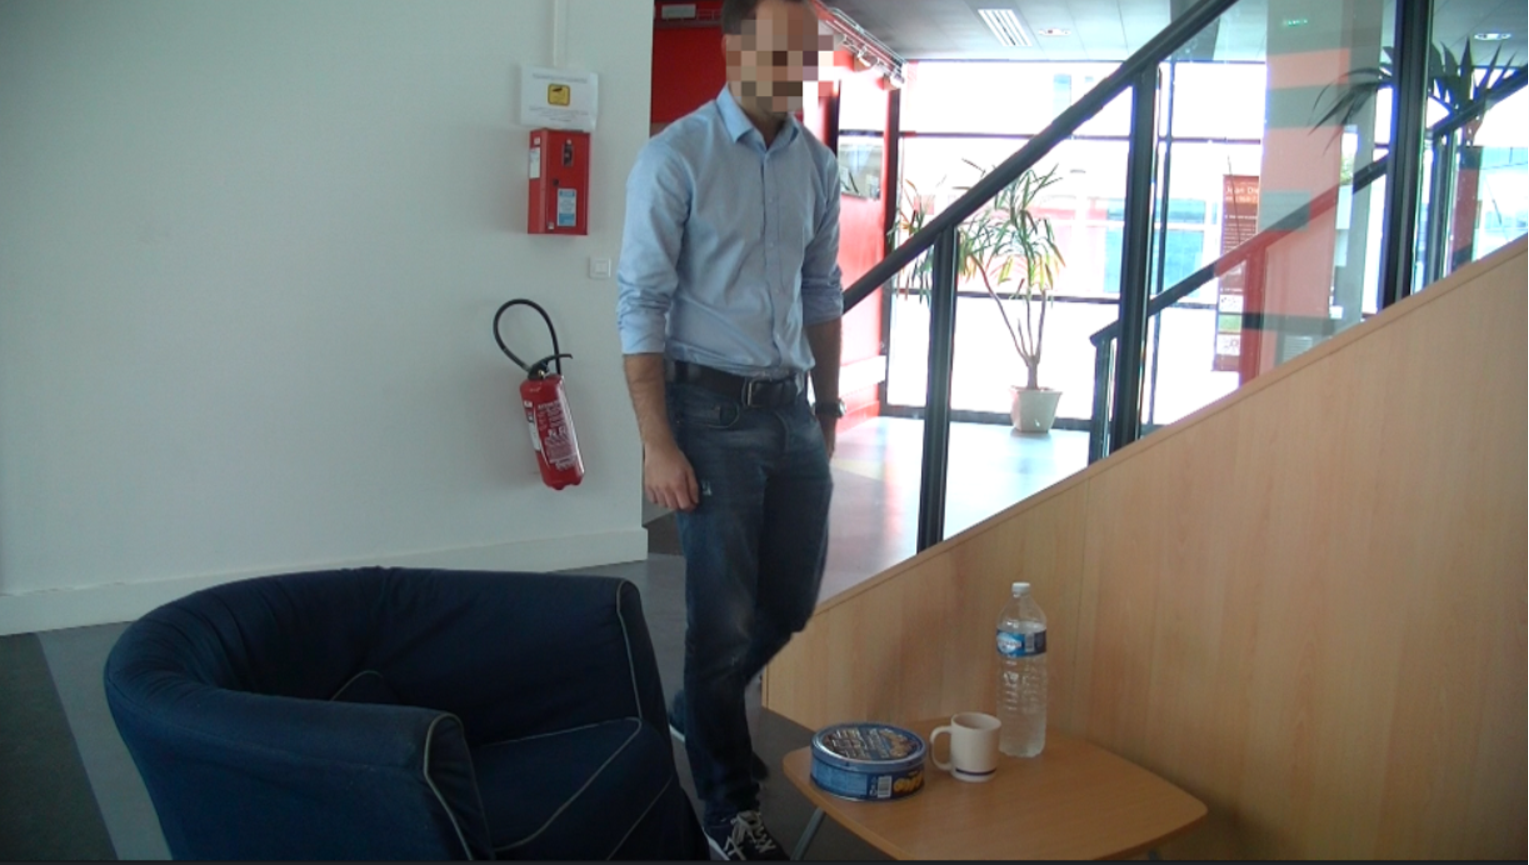
\includegraphics[scale=0.5]{img/observer/cookie1-blur.pdf}
	\caption{The cookie intention scenario}
	\label{fig:observer_experiments-cookie}
\end{figure}


\subsection{Keys Scenario}
\begin{itemize}
\item Objects: A \textit{Box} was placed on the \textit{Table}, that partially occluded the sight of people approaching. A \textit{Book} and a \textit{Mug} where placed behind the \textit{Box}, so that they could be seen from the sofa but not from approaching people.
\item Intentions: \textit{Taking the Mug}, \textit{Taking the Keys}, \textit{Reading the Book}.
\item Tests and Events:
\begin{itemize}
\item \textit{No Clues}: \textit{Max} approaches the \textit{Table}.
\item\textit{Contextual Clues}: \textit{Max} approaches the \textit{Table} in a hurry, while putting on a coat.
\item \textit{Divergent Belief Max}: \textit{Max} approaches the \textit{Table} in a hurry, while putting on a coat.
\end{itemize}
\item \textit{Divergent Belief Event}: \textit{Max} is sitting on the \textit{Table}, drinking from the \textit{Mug}, while having the \textit{Keys} in his hands. His phone rings, so he drops the \textit{Keys} and the \textit{Mug} on the \textit{Table}, behind the \textit{Box}, and leaves the room. While \textit{Max} is away, \textit{Bob} comes and sits on the \textit{Sofa}, reading a \textit{Book}. When he sees the \textit{Keys}, he takes them, places the \textit{Book} on the \textit{Table}, and leaves.
\end{itemize}

The \textit{Divergent Belief Event} was shown to the users (and its simulation streamed to the system) between \textit{Contextual Clues} and the \textit{Divegent Belief Max} events. This scenario can be seen in figure~\ref{fig:observer_experiments-keys}

 \begin{figure}[ht!]
	\centering
	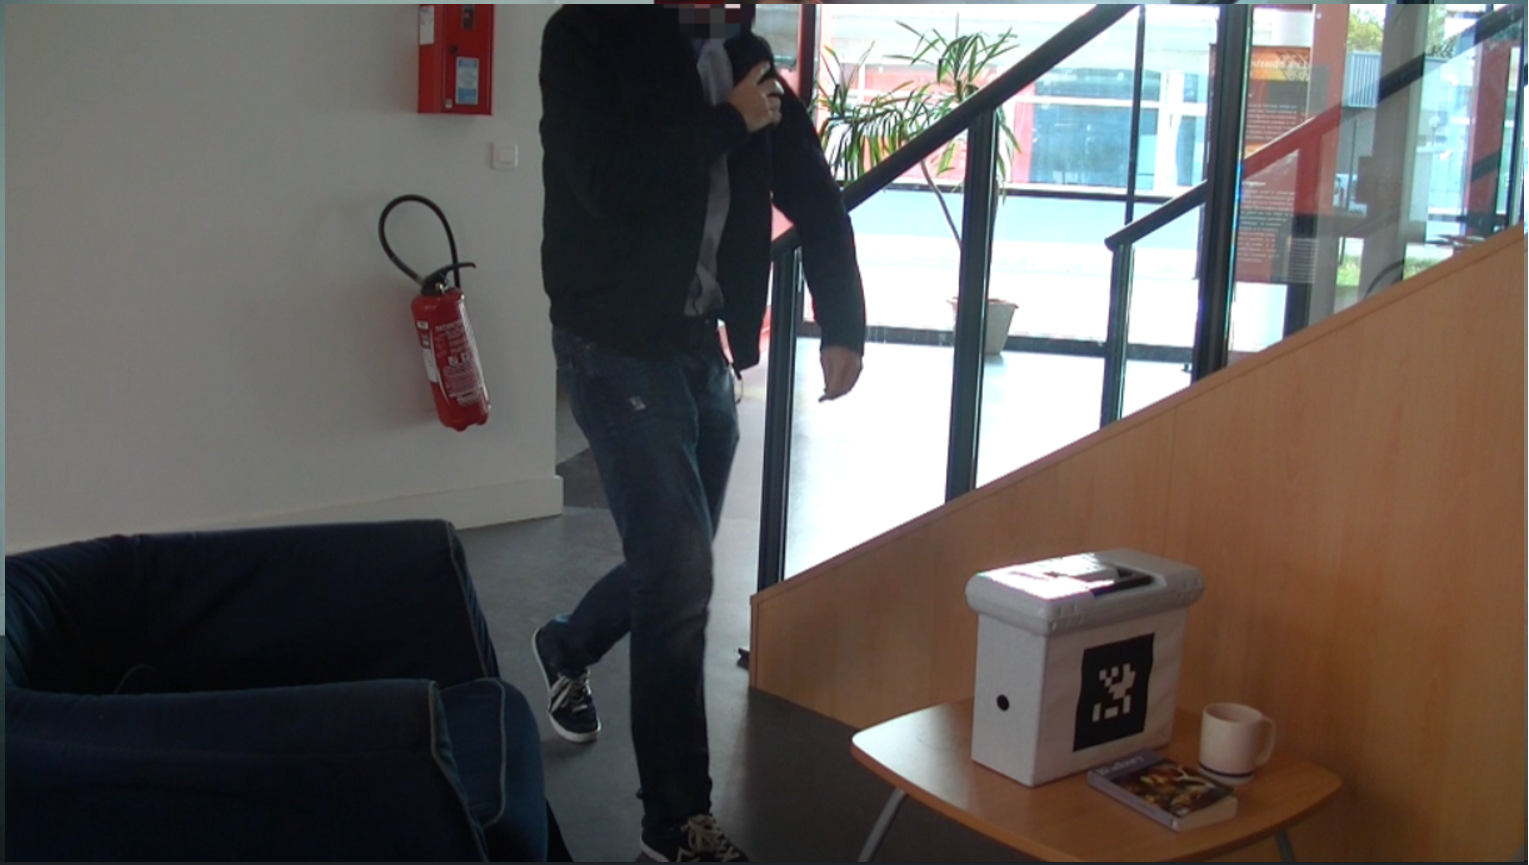
\includegraphics[scale=0.5]{img/observer/keys2-blur.pdf}
	\caption{The keys intention scenario}
	\label{fig:observer_experiments-keys}
\end{figure}

\section{Experiment}
\label{sec:observer_experiment-experiment}
\subsection{User Study}
We built an online user study, where we presented videos related to the tests and events of the two scenarios to users, who had to evaluate the likelihood of each intentions of the scenario
on a five-level Likert scale. The user study was conducted in three languages, with users living in two different countries\footnote{A version of this user study was provided at http://goo.gl/forms/YiuFHnF63c}. We collected answers from 78 adults, performed an average, and converted them to percentile scores, in order to compare them with the system's predictions.

Looking at users' answers (figure \ref{fig:observer_experiments-user_study_results}), we can see that, in the absence of clues, people rated similarly the two intentions related to visible objects. Contextual clues had the highest influence on users' ratings. This is particularly visible in the \textit{Contextual Clues} test of the \textit{Keys Scenario}, where users chose as the most likely intention \textit{Take Keys}, even if no keys were visible in the video. Divergent beliefs also influenced users decisions, but not as strongly as context. The strongest responses, over all, where given by the \textit{Divergent Belief Max} test on \textit{Keys Scenario}, which uses both divergent belief and contextual information.

\subsection{System implementation}
% At the start of a scenario the robot scanned the environment, building a model of its world state. 
We built a simulation related to the scenario, building a world state. With our perception capacities, we would not be able to detect if the cookie box is full or empty, and so we consider it as full at the start of a test, and update its value using the $postconditions$ of inferred human actions. We consider the box as empty when we infer that a human has taken a cookie from inside, and as full when we infer that a human has put a cookie in it.

We have built different IGs for the scenarios. Each test had a different graph, related to its main agent. We considered three different Context Nodes for these IGs: $Hot Day$, true when the day is particularly warm; $Break Time$, true when the agents are taking a pause; $Time to Leave$, true when it's late in the day, and the humans usually leave work and return home.

As previously said, we chose to follow \cite{Liu2014} in order to learn the link between Contexts and Intentions. We created a second user study with 15 users, in which we presented a set of 5 scenarios, each one related to one of the intentions of our tests. For each scenario we asked the users to rate the perceived link, on a five-level Likert scale, between the intention and our three contexts. We averaged users' answers and calculated the conditional probabilities between context nodes and intention nodes from these averages.


In the \textit{Cookie Scenario} the graph for the tests is constructed from the following nodes:
\begin{itemize}
\item Context Nodes: \textit{Hot Day}, \textit{Break Time}, \textit{Time to Leave}
\item Intention Nodes: \textit{Fill Cookie Box}, \textit{Eat Cookie}, \textit{Drink Water}, \textit{Read Book}.
\item Action Nodes: \textit{Move to Table}, \textit{Move to Kitchen}.
\item Observation Nodes: distance of the agent body and hand to each action's associated \textit{target}.
\end{itemize}

We introduce the \textit{Fill Cookie Box} intention, not present in the human test, to allow the system to detect when Bob fills the \textit{Cookie Box} during the \textit{Divergent Belief Event}.

Our system does not have speech recognition capacities. We simulated this capacities, and set Context Nodes to plausible values, that could be extracted by watching the videos. For the \textit{Contextual Clues} test, we set the value of \textit{Hot Day} to true (since Max is commenting about the temperature), and \textit{Break Time}, and \textit{Time to Leave} to false (since no data in the video points to one of these contexts being true. Max and Bob seem to have taken a break from work before the other events are shown, in the Divergent Belief Event).
%Our robot doesn't have speech recognition capacities. and for \textit{Contextual Clues} test, set the value of \textit{Hot Day} to \textit{true}, and the value of \textit{Break Time} to \textit{false}, i.e. the robot knows that it is not the usual time for the agents to take a break.

\textit{Divergent Belief Event}, \textit{Divergent Belief Max}, and \textit{Divergent Belief Bob} were streamed sequentially to the system, which updated the agents' mental models and created new IGs accordingly. During the \textit{Divergent Belief Event} several IGs need to be created with different Action and Observation nodes, to follow the sequence of actions by the two agents. For example, when \textit{Max} leaves the room, \textit{Bob} has the possibility to execute the actions \textit{Take Mug}, \textit{Take Water Bottle}, \textit{Open Cookie Box}, \textit{Move to Kitchen Shelf} or \textit{Leave Room}. Intention and Context nodes remains the same in all the IGs of the scenario.


The \textit{Keys Scenario} has a similar IG, with the following differences.
\begin{itemize}
\item Context Nodes: \textit{Hot Day}, \textit{Break Time} and \textit{Time to Leave}.
\item Intention Nodes: \textit{Drink Water}, \textit{Take Keys}, \textit{Read Book}.
\end{itemize}

Action Nodes and Observation Nodes are the same as the previous scenario, and follow the same ideas during the \textit{Divergent Belief Event}. An example of IG used in the tests can be seen in figure \ref{fig:observer_experiments-intention_graph}. For the \textit{Contextual Clues} and \textit{Divergent Belief} test, we set the \textit{Time to Leave} context value to \textit{true} (since Max is putting a coat and seems in a hurry), and other context node values to \textit{false}. Using the component described in the previous sections, and these IGs the system was able to obtain predictions from the user actions.

\section{Discussion}
\label{sec:observer_experiment-discussion}
We performed TOST tests for each intention in the scenarios, comparing the humans' answers with the system's, for a total of 21 tests. We calculated p-values and performed our tests using a significance value $\alpha=0.05$.

Analyzing the results of our equivalence tests, shown in figure \ref{fig:observer_experiments-user_study_results}, produces some interesting information.
\begin{itemize}
\item The behavior of our system is often close to human capacities. 19 tests out of 21 passed our requirements for significance level, often with very low p-value scores. 
\item Context and Divergent Belief are necessary. A system without these skills would only have been able to model properly the \textit{No Clues} cases. 
\item There are still some missing aspects in our system. We failed to reject the null hypothesis for two tests. In \textit{Divergent Belief Bob} users rated higher the \textit{Eat Cookie} intention than the \textit{Drink Water} intention, possibly because they thought that since \textit{Bob} filled the \textit{Cookie Box} he may want to eat a \textit{Cookie}. This makes us think that humans use deep temporal reasoning to evaluate intentions, considering the whole history of actions performed by agents.  
\end{itemize}
 \begin{figure}[ht!]
	\centering
	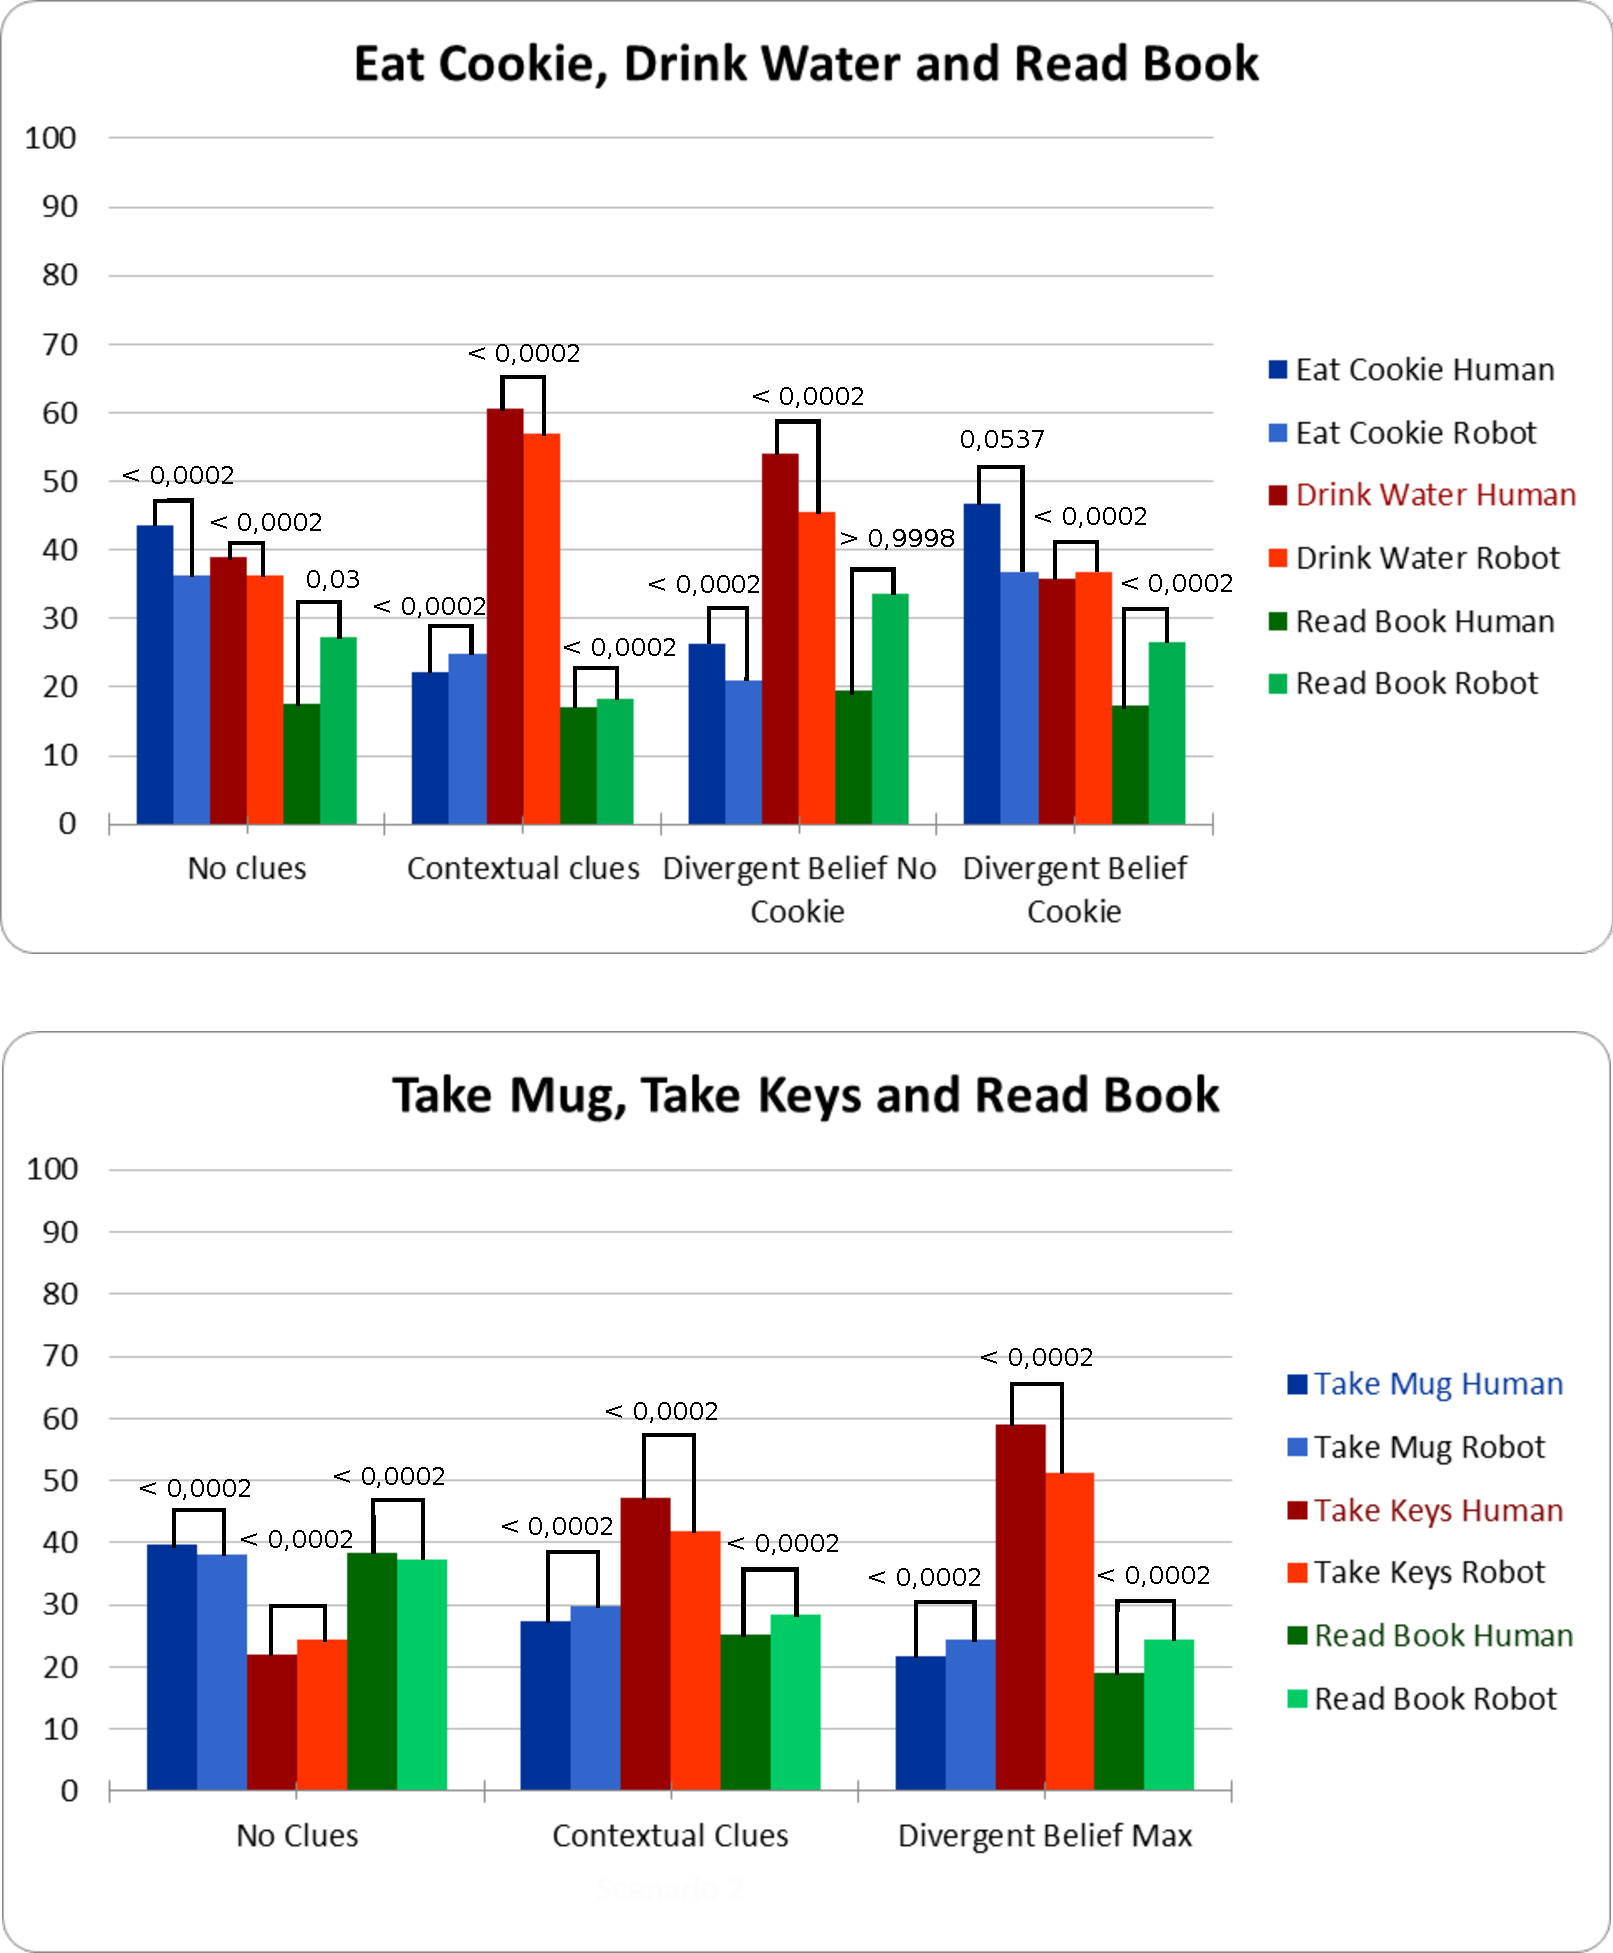
\includegraphics[clip,scale=0.5]{img/observer/pvalues1.pdf}
	\caption[Experiment results]{Experiment results. Results from the two scenarios are represented as graphs. Intentions, as estimated by the humans and the system (called Robot in the image) as , are represented by different colors, as shown in the legend of the graphs, with estimations of the same intention by the system or the human placed in adjacent position. Each column represents the likelihood of an intention, expressed as a percentile score. P-values from the equivalence tests are shown, linking the estimation of an intention by the humans and by the system.}
	\label{fig:observer_experiments-user_study_results}
\end{figure}



